\section{Transformée de Fourier rapide}

La FFT (\textit{Fast Fourier Transform}, transformée de Fourier rapide) désigne une famille d'algorithmes permettant de calculer \og rapidement \fg la transformée de Fourier discrète d'un signal. En particulier, la complexité temporelle des algorithmes FFT est en $\Theta \left(n \log \left( n \right) \right)$, ces algorithmes sont donc bien plus efficaces que l'algorithme naïf, consistant à appliquer directement la définition de la TFD et dont la complexité est en $\Theta\left( n^2 \right)$.

Les premières ébauches de FFT remontent au début du XIX\textsuperscript{ème} siècle, Gauss en avait alors imaginé le principe\cite{gauss-fft} mais le concept a réellement connu un regain d'intérêt dans la deuxième moitié du XX\textsuperscript{ème} siècle avec l'essor de l'informatique.

\subsection{Algorithme de Cooley-Tukey}
\label{section-cooley-tukey}

En 1965, les mathématiciens James Cooley et John Tukey publient un article présentant un algorithme de FFT appelé algorithme de Cooley-Tukey\cite{cooley-tukey-fft} qui relance l'intérêt pour la transformée de Fourier rapide. Il s'agit dans sa version la plus simple d'un algorithme récursif.

Dans un premier temps, il faut reformuler quelque peu les termes du problème\cite{algo-fft}. On a vu précédemment que la TFD d'un signal $x = \left( x_0, \dots, x_{N - 1} \right)$ était le vecteur $X = \left( X_0, \dots, X_{N-1} \right)$ avec $X_k = \sum_{n = 0}^{N - 1} x_n e^{-i \frac{2 \pi}{N} k n}$. Or, si on pose $P = \sum_{n=0}^{N - 1} x_n X^n$ et $\omega_N = e^{-i \frac{2 \pi}{N}}$ une racine primitive $N$-ième de l'unité, alors, calculer $X_k$ revient à évaluer $P$ en ${\omega_N}^k = e^{-i \frac{2 \pi}{N} k}$. On suppose dans la suite que $N$ est une puissance de 2.
On peut alors exploiter cette reformulation pour réduire le coût de calcul, on va décomposer $P$ en deux polynômes de degré inférieur. En particulier, on a,
\begin{align*}
P(X) &= \sum_{n=0}^{N-1} x_n X^n \\
&= \sum_{n=0}^{\frac{N}{2}-1} x_{2n} X^{2 n} + \sum_{n=0}^{\frac{N}{2}-1} x_{2 n + 1} X^{2 n + 1} \\
&= \sum_{n=0}^{\frac{N}{2}-1} x_{2 n} (X^2)^n + X \sum_{n=0}^{\frac{N}{2}-1} x_{2 n + 1} (X^2)^n
\end{align*}

On pose alors,
$$
P_{\text{pair}}(X) = \sum_{n=0}^{\frac{N}{2}-1} x_{2 n} X^n \quad \text{et} \quad P_{\text{impair}}(X) = \sum_{n=0}^{\frac{N}{2}-1} x_{2 n + 1} X^n
$$
on obtient finalement,
$$
P(X) = P_{\text{pair}}(X^2) + X P_{\text{impair}}(X^2)
$$

Ainsi, pour $k \in \{0, \dots, N - 1\}$,
$$
X_k = P({\omega_N}^k) = P_{\text{pair}}({\omega_N}^{2 k}) + {\omega_N}^k P_{\text{impair}}({\omega_N}^{2 k}).
$$

Or, ${\omega_N}^{2} = e^{-i \frac{4 \pi}{N}} = e^{-i \frac{2\ pi}{N / 2}} = {\omega_{N / 2}}$ et $P_{\text{pair}}$ et $P_{\text{impair}}$ sont de degré $\tfrac{N}{2}$. Ainsi, les termes $P_{\text{pair}}({\omega_N}^{2 k})$ et $P_{\text{impair}}({\omega_N}^{2 k})$ correspondent à des transformées de Fourier discrètes de taille $\tfrac{N}{2}$.

On obtient donc les relations suivantes, pour $k \in \{0, \dots, \frac{N}{2}-1\}$ :
$$
X_k = E_k + {\omega_N}^k O_k, \quad X_{k + \frac{N}{2}} = E_k - {\omega_N}^k O_k
$$
où
$$
E_k = P_{\text{pair}}({\omega_N}^{2 k}), \quad O_k = P_{\text{impair}}({\omega_N}^{2 k})
$$

Cette décomposition permet de calculer une TFD de taille $N$ à partir de deux TFD de taille $\tfrac{N}{2}$. On observe en outre que si $N = 1$, on a $X_0 = \sum_{n=0}^{0} x_0 e^{-i \frac{2 \pi}{N} \cdot 0 \cdot n} = x_0$. On en déduit l'algorithme récursif suivant :

\begin{algorithm}[H]
\DontPrintSemicolon
\Donnees{Un signal $x = \left( x_0, \dots, x_{N-1} \right)$ et la racine de l'unité $\omega = e^{-i \frac{2 \pi}{N}}$.}

\Resultat{La transformée de Fourier discrète du signal $x$, $X = \left( X_0, \dots, X_{N-1} \right)$.}
\SetKwFunction{FFT}{fft}
\SetKwProg{Fn}{Fonction}{:}{}

\Fn{\FFT{$x, \omega$}}{
    \Si{$N = 1$}{
        \Retour $\left( x_0 \right)$\;
    }\Sinon{
        $E \gets $ \FFT{$\left( x_0, x_2, \dots, x_{N - 2} \right), \omega^2$}\;
        $O \gets $ \FFT{$\left( x_1, x_3, \dots, x_{N - 1} \right), \omega^2$}\;
        $\alpha \gets 1$\;

        \Pour{$k = 0$ \KwTo $\frac{N}{2} - 1$}{
            $X_k \gets E\left[ k \right] + \alpha \times O\left[ k \right]$\;
            $X_{k + \frac{N}{2}} \gets E\left[ k \right] - \alpha \times O\left[ k \right]$\;
            $\alpha \gets \alpha \times \omega$\;
        }
        \Retour $\left( X_0, \dots, X_{N - 1} \right)$\;
    }
}

\caption{Algorithme de Cooley-Tukey\cite{algo-fft}}
\end{algorithm}

Notons que la racine de l'unité $\omega$ est donnée en entrée de la fonction \FFT, on évite ainsi de la recalculer en fonction de $N$ à chaque appel récursif. En pratique une fonction \textit{wrapper} (enveloppante), ne prenant pas $\omega$ en paramètre, se chargera de calculer $\omega_N$ avant d'appeler \FFT une première fois.

\hyperref[exemple-cooley]{Voir une décomposition d'un appel en annexe}.

\subsection{Complexité algorithmique}

L'algorithme de Cooley-Tukey a une complexité algorithmique en $\Theta \left( n \log \left( n \right) \right)$ où $n$ est la taille du signal à traiter. Ce résultat se démontre à l'aide du \textit{master theorem}\cite{wiki-master-theorem} (aussi appelé \og théorème sur les récurrences par partition \fg). 

En effet, si on note $\tau \left( n \right)$ le nombre d'opérations élémentaires pour exécuter \FFT sur un signal de longueur $n$, on a,
\begin{align*}
\tau \left( n \right) &= 2 \tau \left( \frac{n}{2} \right) + \Theta \left( n \right) \\
&= a \tau \left( \frac{n}{b} \right) + f \left( n \right) \quad \text{avec $a = b = 2$ et $f \left( n \right) = \Theta \left( n \right)$}
\end{align*}
On calcule alors,
$$
n^{\log_b{a}} = n^{\log_2{2}} = n^1 = n
$$
On obtient,
$$
f \left( n \right) = \Theta \left( n \right) = \Theta \left( n^{\log_b{a}} \right)
$$
On en déduit donc, d'après le \textit{master theorem}, que $\tau \left( n \right) = \Theta \left( n^{\log_b{a}} \log \left( n \right) \right) = \Theta \left( n \log \left( n \right) \right)$.


\subsection{Approche itérative}
\label{section-approche-iterative}

Bien que l'implémentation fidèle de l'algorithme de Cooley-Tukey décrit précédemment se révèle bien plus efficace que l'algorithme naïf, issu de la définition de la TFD, il reste très lent comparé à l'implémentation de référence pour Python fournie dans le module numpy.

Il est néanmoins possible d'améliorer notre implémentation en abandonnant l'approche récursive au profit d'une approche itérative\cite{implementation-fft}. Cela nous permettra de supprimer les copies et allocations de tableaux et éviter les coûts supplémentaires, en temps et en mémoire, liés à la récursion.

L'idée centrale consiste à simuler les appels récursifs \og du bas vers le haut \fg . Le problème, pour accomplir cela, est que l'on ne sait pas, à priori, comment recomposer les sous-tableaux en partant de l'étape avec $N$ sous-tableaux de taille 1. En réalité, le découpage des sous-tableaux en indices pairs/impairs à chaque étape de la récursion permet de \og lire \fg , dans l'écriture binaire des indices des éléments, leur parcours dans les différents sous-tableaux.

Plus précisément, si le tableau à traiter a pour longueur $2^m$, on peut représenter l'indice $k$ d'un élément $x$ en binaire $k = \overline{b_{m - 1}b_{m - 2}\dots b_0}^2$. Alors, lors du premier appel, $x$ est placé dans le sous-tableau pair ou impair en fonction de la parité de $b_0$. Lors du deuxième appel, tous les éléments placés avec $x$ ont la même valeur pour $b_0$, ainsi séparer éléments pairs et impairs se fait en regardant le bit $b_1$. Ce processus se poursuit jusqu'à obtenir des sous-tableaux de taille 1. Ainsi, en partant des sous-tableaux de taille 1, les recompositions à faire se déduisent de la suite $\left( b_0, b_1, \dots, b_{m - 1} \right)$.

À partir de ce constat, on peut obtenir la version itérative de l'algorithme. On commence par réorganiser le tableau en entrée en inversant l'ordre des bits des indices. Une fois le tableau réordonné, on applique les opérations papillons de manière itérative. Une boucle, faisant $\log_2 \left( N \right)$ tours, remplace les appels récursifs. À l'étape $j$, on combine des blocs de taille $2^j$. On en déduit l'algorithme itératif suivant :


\begin{algorithm}
\DontPrintSemicolon
\Donnees{Un signal $x = (x_0, \dots, x_{N-1})$.}

\Resultat{La transformée de Fourier discrète du signal $X = (X_0, \dots, X_{N-1})$.}

\SetKwFunction{FFTITER}{fft\_iterative}
\SetKwFunction{BITREVERSE}{bit\_reversal\_permutation}
\SetKwProg{Fn}{Fonction}{:}{}

\Fn{\FFTITER{$x$}}{
    $x \gets \BITREVERSE(x)$\;

    $t \gets 1$\;
    $m \gets 2$\;

    \Pour{$j = 1$ \KwTo $\log_2 N$}{
        $\omega_m \gets e^{\frac{-2 i \pi}{m}}$\;
        $\alpha \gets 1$\;

        \Pour{$l = 0$ \KwTo $t - 1$}{
            \Pour{$k = l$ \KwTo $N - 1$ \KwBy $m$}{
                $u \gets x_k$\;
                $v \gets \alpha \times x_{k + t}$\;
                $x_k \gets u + v$\;
                $x_{k + t} \gets u - v$\;
            }

            $\alpha \gets \alpha \times \omega_m$\;
        }

        $t \gets m$\;
        $m \gets 2 \times m$\;
    }

    \Retour $(x_0, \dots, x_{N-1})$\;
}

\caption{Algorithme de Cooley-Tukey itératif}
\end{algorithm}

Cette version itérative a de meilleures performances que notre première version récursive, en revanche elle reste loin de l'efficacité de l'implémentation de numpy (\hyperref[compilation-jit]{Voir comment réduire drastiquement cet écart en annexe}).

\begin{figure}[H]
    \centering
    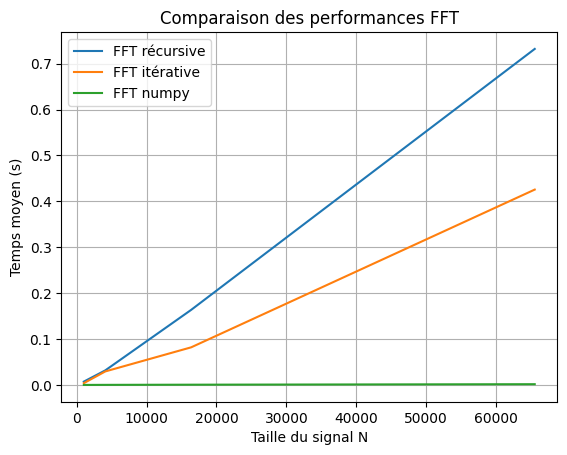
\includegraphics[width=0.6\textwidth]{images/FFT_performances.png}
    \caption{Temps de calcul moyen en fonction de la taille du signal pour différentes FFT.}
\end{figure}

\subsection{Spectre de la FFT}
\label{section-spectre-fft}

\begin{figure}[H]
    \centering
    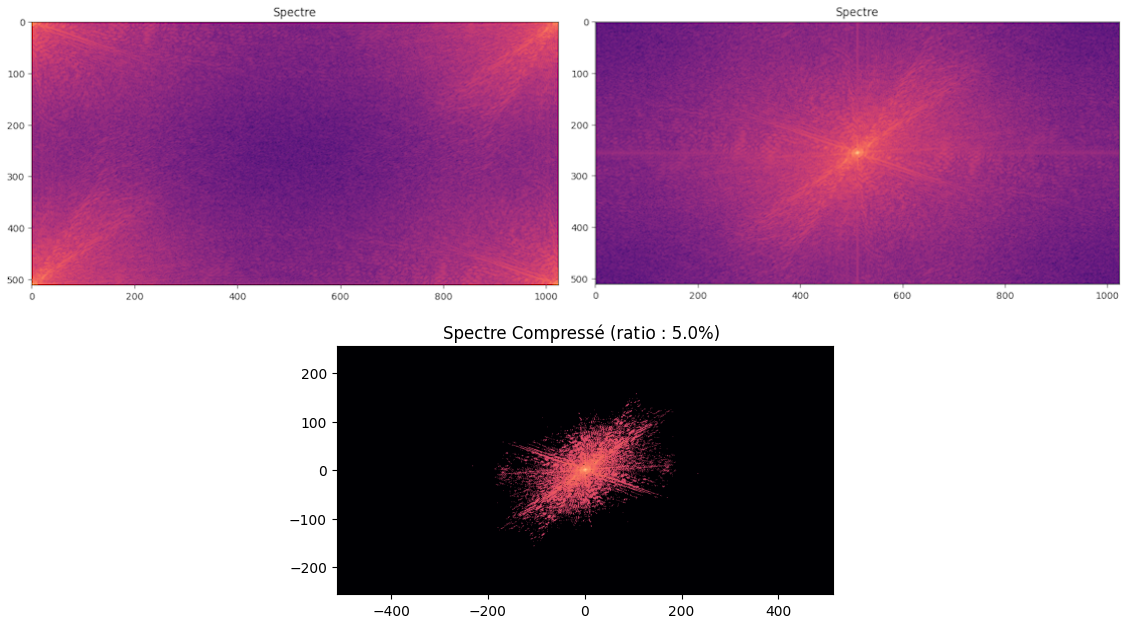
\includegraphics[width=0.75\textwidth]{images/Spectres_FFT.png}
    \caption{Analyses du spectre obtenu par FFT}
\end{figure}
Sur la première figure, on observe le spectre de l'image après application de la FFT. La couleur est donnée par la formule $c = \ln(1+a_{k,l})$ pour éviter que les valeurs n'explosent. On observe que les valeurs les plus importantes, les basses fréquences sont réparties dans les coins du spectre (\hyperref[preuve-spectre-fft]{Voir la démonstration en annexe}). On peut alors réaliser une opération appelée \textbf{Shift} pour replacer les basses fréquences au centre du spectre. Pour ce faire, on échange le coin supérieur gauche avec celui inférieur droit et celui supérieur droit avec celui inférieur gauche. La deuxième figure représente le spectre obtenu après un Shift. Les basses fréquences sont concentrées au centre du spectre. La dernière figure, représente le spectre compressé en ne gardant que 5\% des coefficients de la matrice du spectre. Le fait de ne garder qu'une partie des coefficients pour compresser une image sera détaillé lorsque nous analyserons la Transformée en cosinus discrète par la suite. \\
Pour compresser l'image, il suffit de trier les coefficients en fonction de leur fréquence et ne garder qu'un certain nombre de coefficients en gardant les basses fréquences car elles permettent de garder les détails principaux de l'image originale (\hyperref[preuve-compression-fft]{Voir la démonstration en annexe}).
